\documentclass[12pt]{article}
\usepackage{geometry}
\geometry{a4paper, margin=1in}
\usepackage{graphicx}
\usepackage{titlesec}
\usepackage{xcolor}
\usepackage{hyperref}
\usepackage{fancyhdr}
\usepackage{enumitem}

% Formatting
\titleformat{\section}{\large\bfseries}{\thesection.}{0.5em}{}
\pagestyle{fancy}
\setlength{\headheight}{15pt}
\fancyhf{}
\rhead{EE175A/B - Weekly Progress Report}
\lhead{Battery Management and Communication System}
\rfoot{Page \thepage}

\begin{document}

\begin{center}
    {\Large \textbf{Weekly Progress Report (WPR)}} \\[6pt]
    {\large \textbf{Battery Management and Communication System (BMS)}} \\[2pt]
    \rule{0.8\textwidth}{0.5pt} \\[6pt]
\end{center}

\noindent
\textbf{Team:} Kaushik Vada, Christian Kim, Connor Stewart, Nick Poon \\[3pt]
\textbf{Course:} EE175B - Senior Design II \\
\textbf{Instructor:} Prof. Roman Chomko \\
\textbf{Week:}(\textit{Feb 9 - Feb 15, 2026}) \\[8pt]

\vspace{1em}

\section{Work Completed This Week}
\begin{itemize}[leftmargin=1cm]
    \item Built a complete desktop release pipeline using GitHub Actions for Windows, macOS, and Linux, including automated artifact publishing, code signing for macOS, and stable download links.
    \item Implemented an in-app auto-updater with download progress indicators and seamless installer handoff, hardened across all three platforms (Windows NSIS, macOS DMG, Linux AppImage).
    \item Developed serial data stream parsing to support both JSON and firmware text frames (V/T/I telemetry), enabling real-time data visualization from the STM32 firmware to the GUI.
    \item Made the BMS Dashboard GUI fully responsive and adaptive across different screen sizes and resolutions.
    \item Added a simulation data toggle feature with safe mode switching, allowing the GUI to be tested independently of hardware connections.
    \item Designed and implemented a cinematic boot-to-dashboard startup transition with a liquid glass boot loader animation for polished user experience.
    \item Flashed and tested USB-Connection-Firmware on the STM32F303RC, integrating HAL driver libraries and middleware for USB device communication.
    \item Fixed multiple GUI bugs including camera zoom issues in simulation mode, boot transition flickering, and simulation toggle visual feedback.
    \item Released multiple application versions from v0.1.1 through v2.0.1, iteratively improving stability, performance, and cross-platform compatibility.
\end{itemize}

\vspace{1em}

\section{Challenges Encountered}
\begin{itemize}[leftmargin=1cm]
    \item Resolving Windows updater handoff issues where the installer needed to launch after the application fully exits, requiring multiple iterations to harden the lock handling and close flow.
    \item macOS code signing and notarization caused ``app is damaged'' errors after bundle modification, requiring re-signing of the application bundle post-build.
    \item Handling monorepo long-path checkout failures in the GitHub Actions release workflow, solved by implementing sparse checkout.
    \item Ensuring the serial parser reliably handles mixed JSON and raw firmware text frames without data corruption or partial packet reads.
\end{itemize}

\vspace{1em}

\section{Work Plan for Next Week}
\begin{itemize}[leftmargin=1cm]
    \item Verify all physical and electrical connections on the BMS and E-Load boards for hardware validation.
    \item Establish a stable end-to-end live data stream from the BMS firmware through USB to the desktop GUI application.
    \item Begin implementing Fault Management System (FMS) logic and integrate fault alerts into the GUI dashboard.
    \item Continue iterating on firmware to support additional sensor readings and E-Load control commands.
\end{itemize}

\vspace{1em}

\section{Appendix A - System Block Diagram}
\begin{center}
    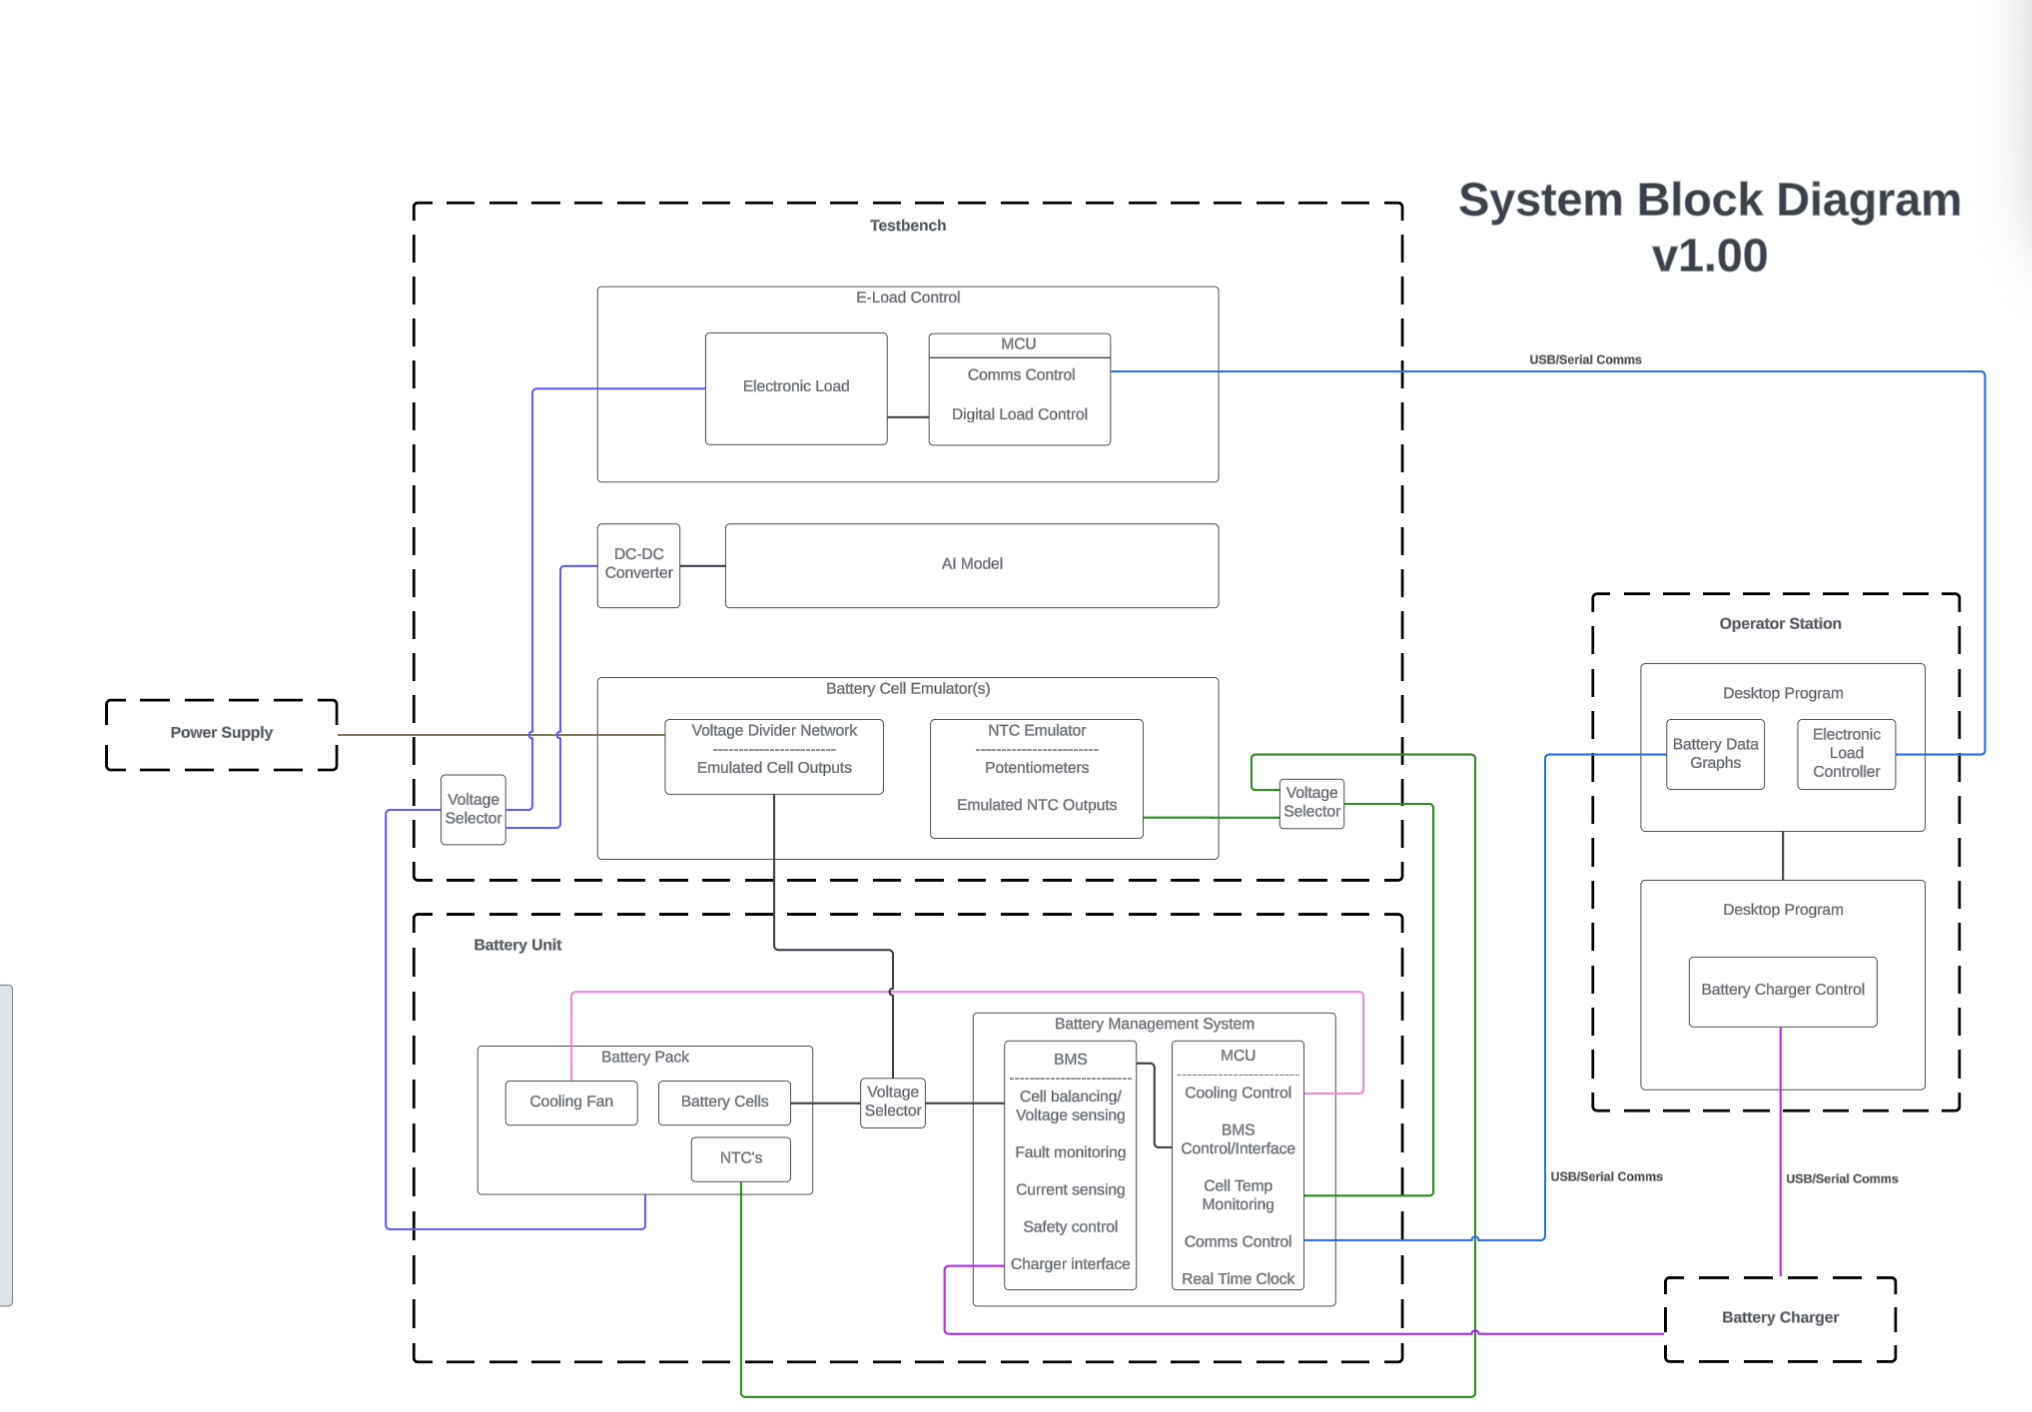
\includegraphics[width=0.95\textwidth]{bms_block_diagram.png} [Figure 1]
\end{center}
\noindent
\textit{Figure A1:} Updated System Block Diagram showing battery domain, isolation components, STM32 communication, and host interface (Source: EE175 Project Report).

\vspace{1em}

\section{Appendix B - Enclosure Visualization}
\begin{center}
    \includegraphics[width=0.95\textwidth]{BMS_enclosure.png} [Figure 2]
\end{center}
\noindent
\textit{Figure B1:} 3D rendering of BMS enclosure with semi-transparent lid, showing airflow, fan, USB-C port, and internal component placement.

\vspace{1em}

\section{Appendix C - Battery Pack Implementation}
\begin{center}
    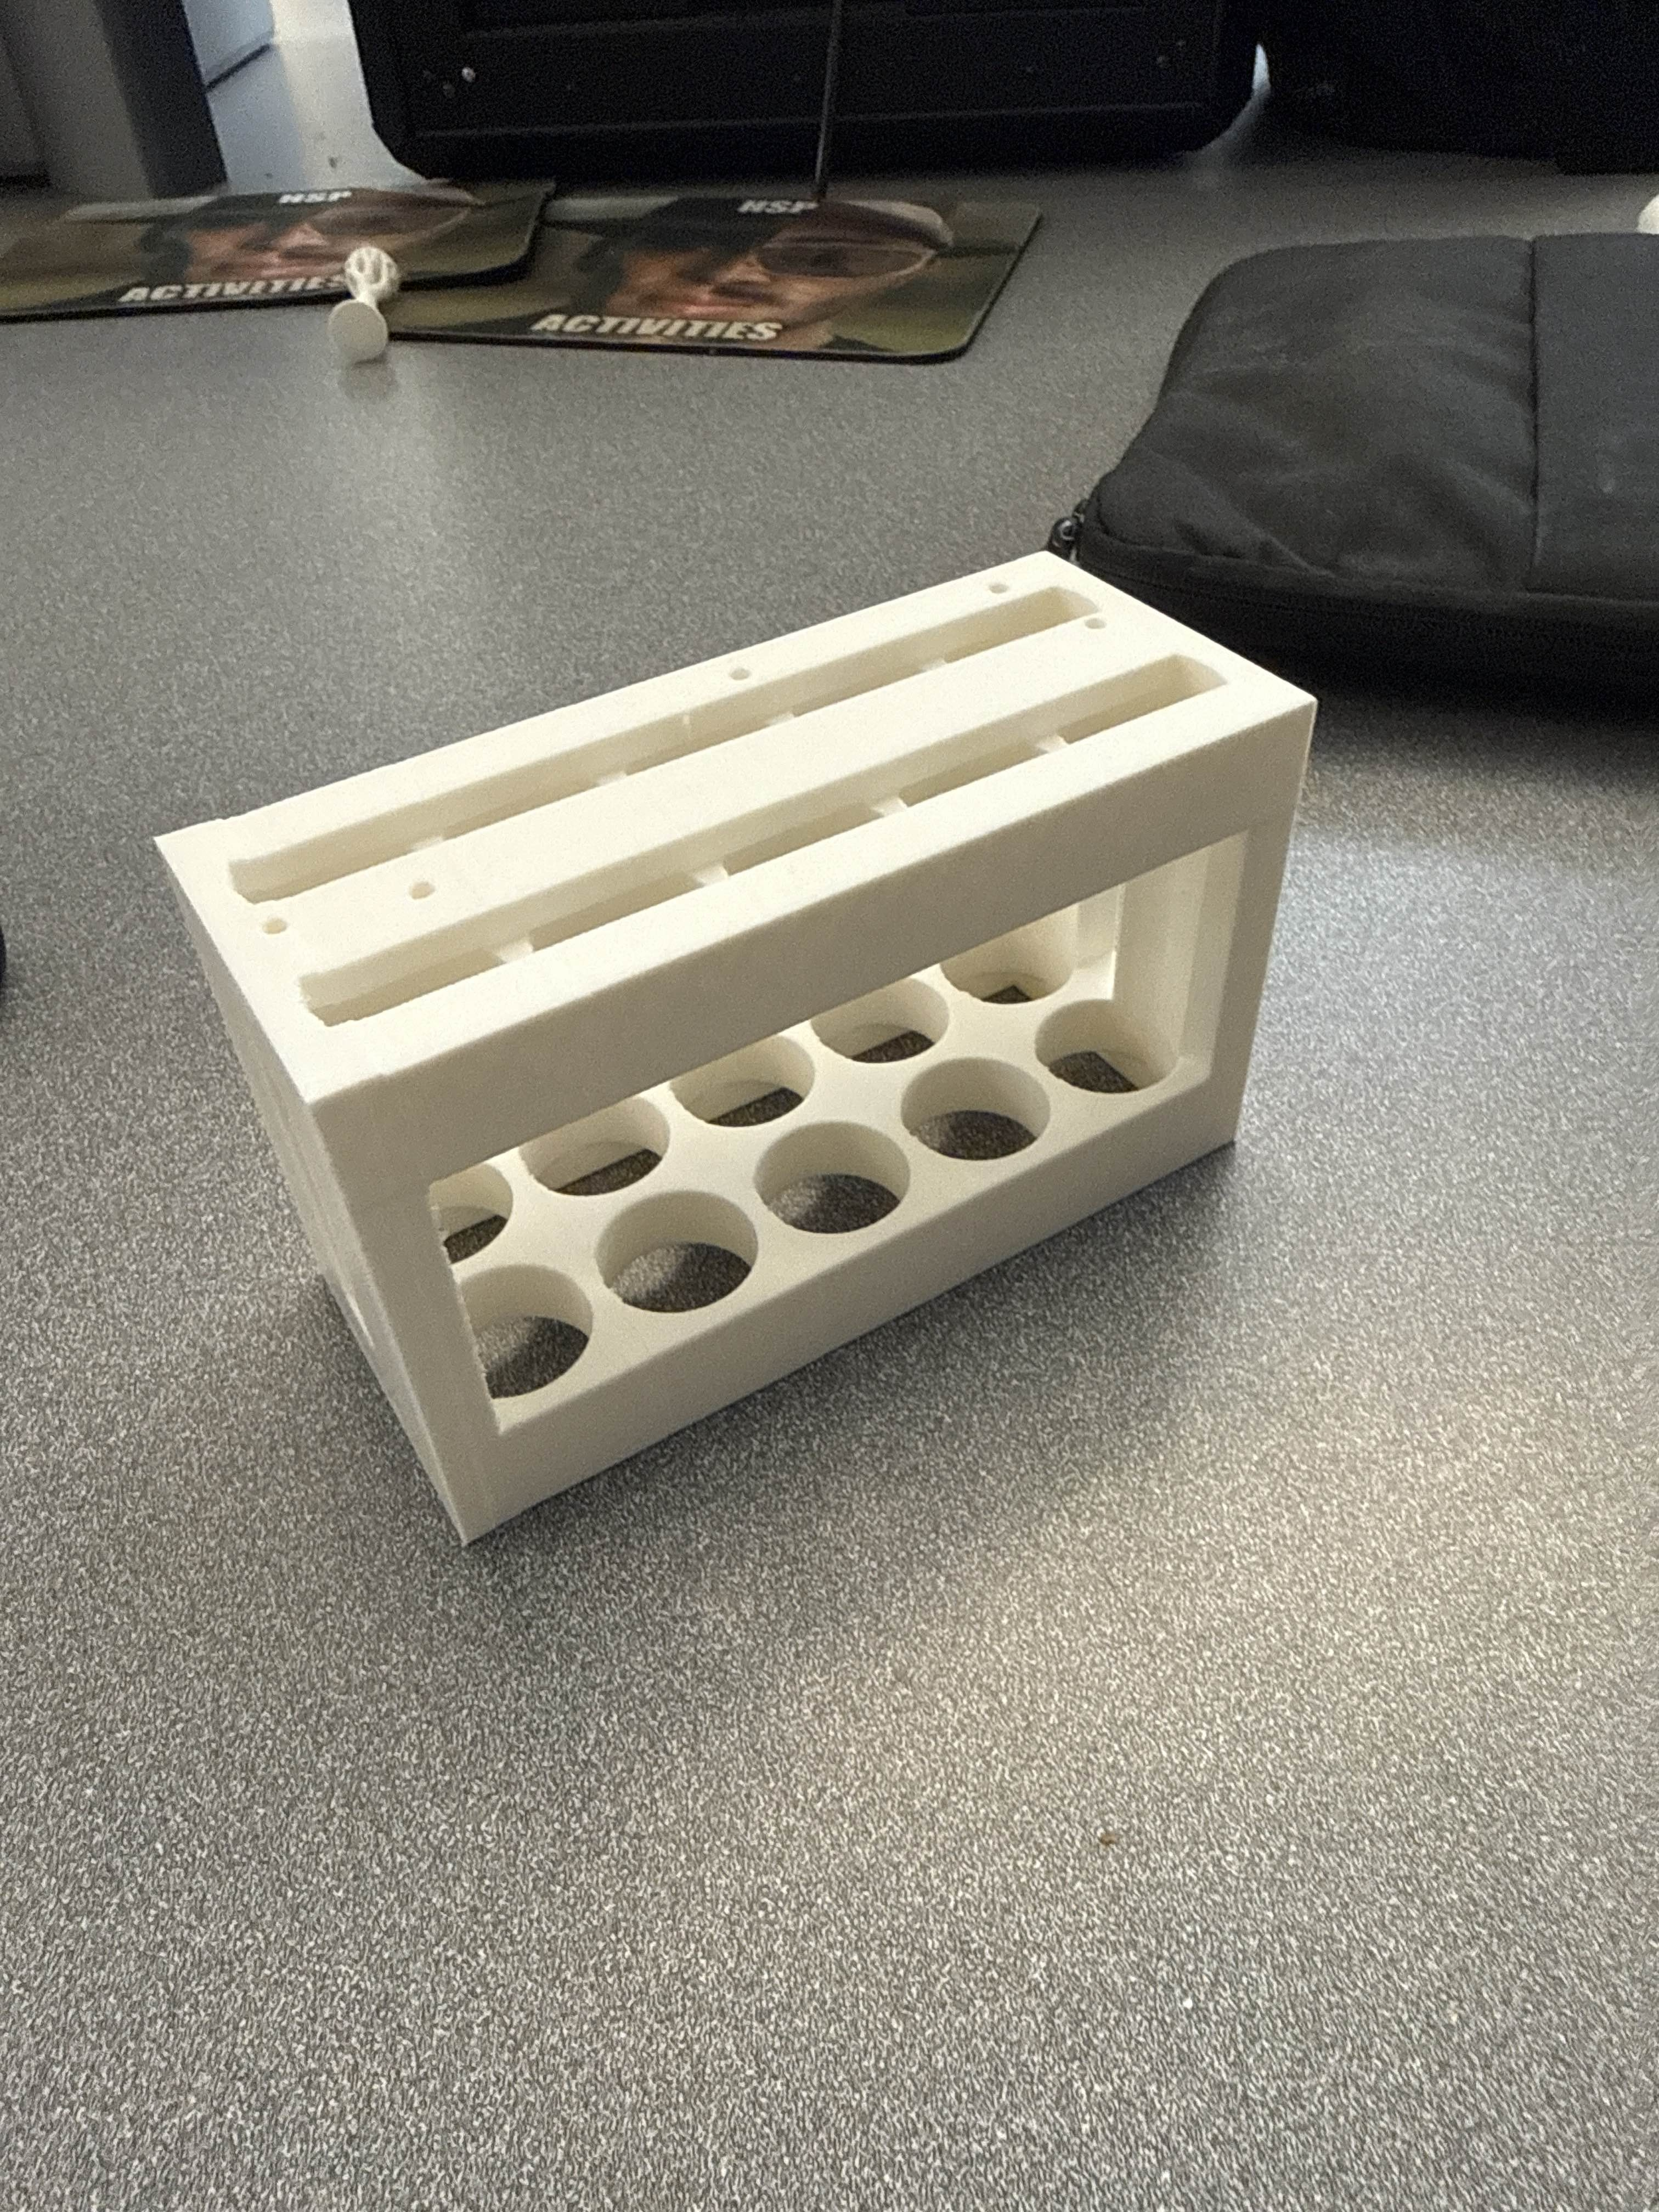
\includegraphics[width=0.95\textwidth]{Battery_Pack.png} [Figure 3]
\end{center}
\noindent
\textit{Figure C1:} Battery pack assembly showing cell arrangement and integration with the BMS unit.

\vspace{1em}

\section{Appendix D - BMS GUI Visualization}
\begin{center}
    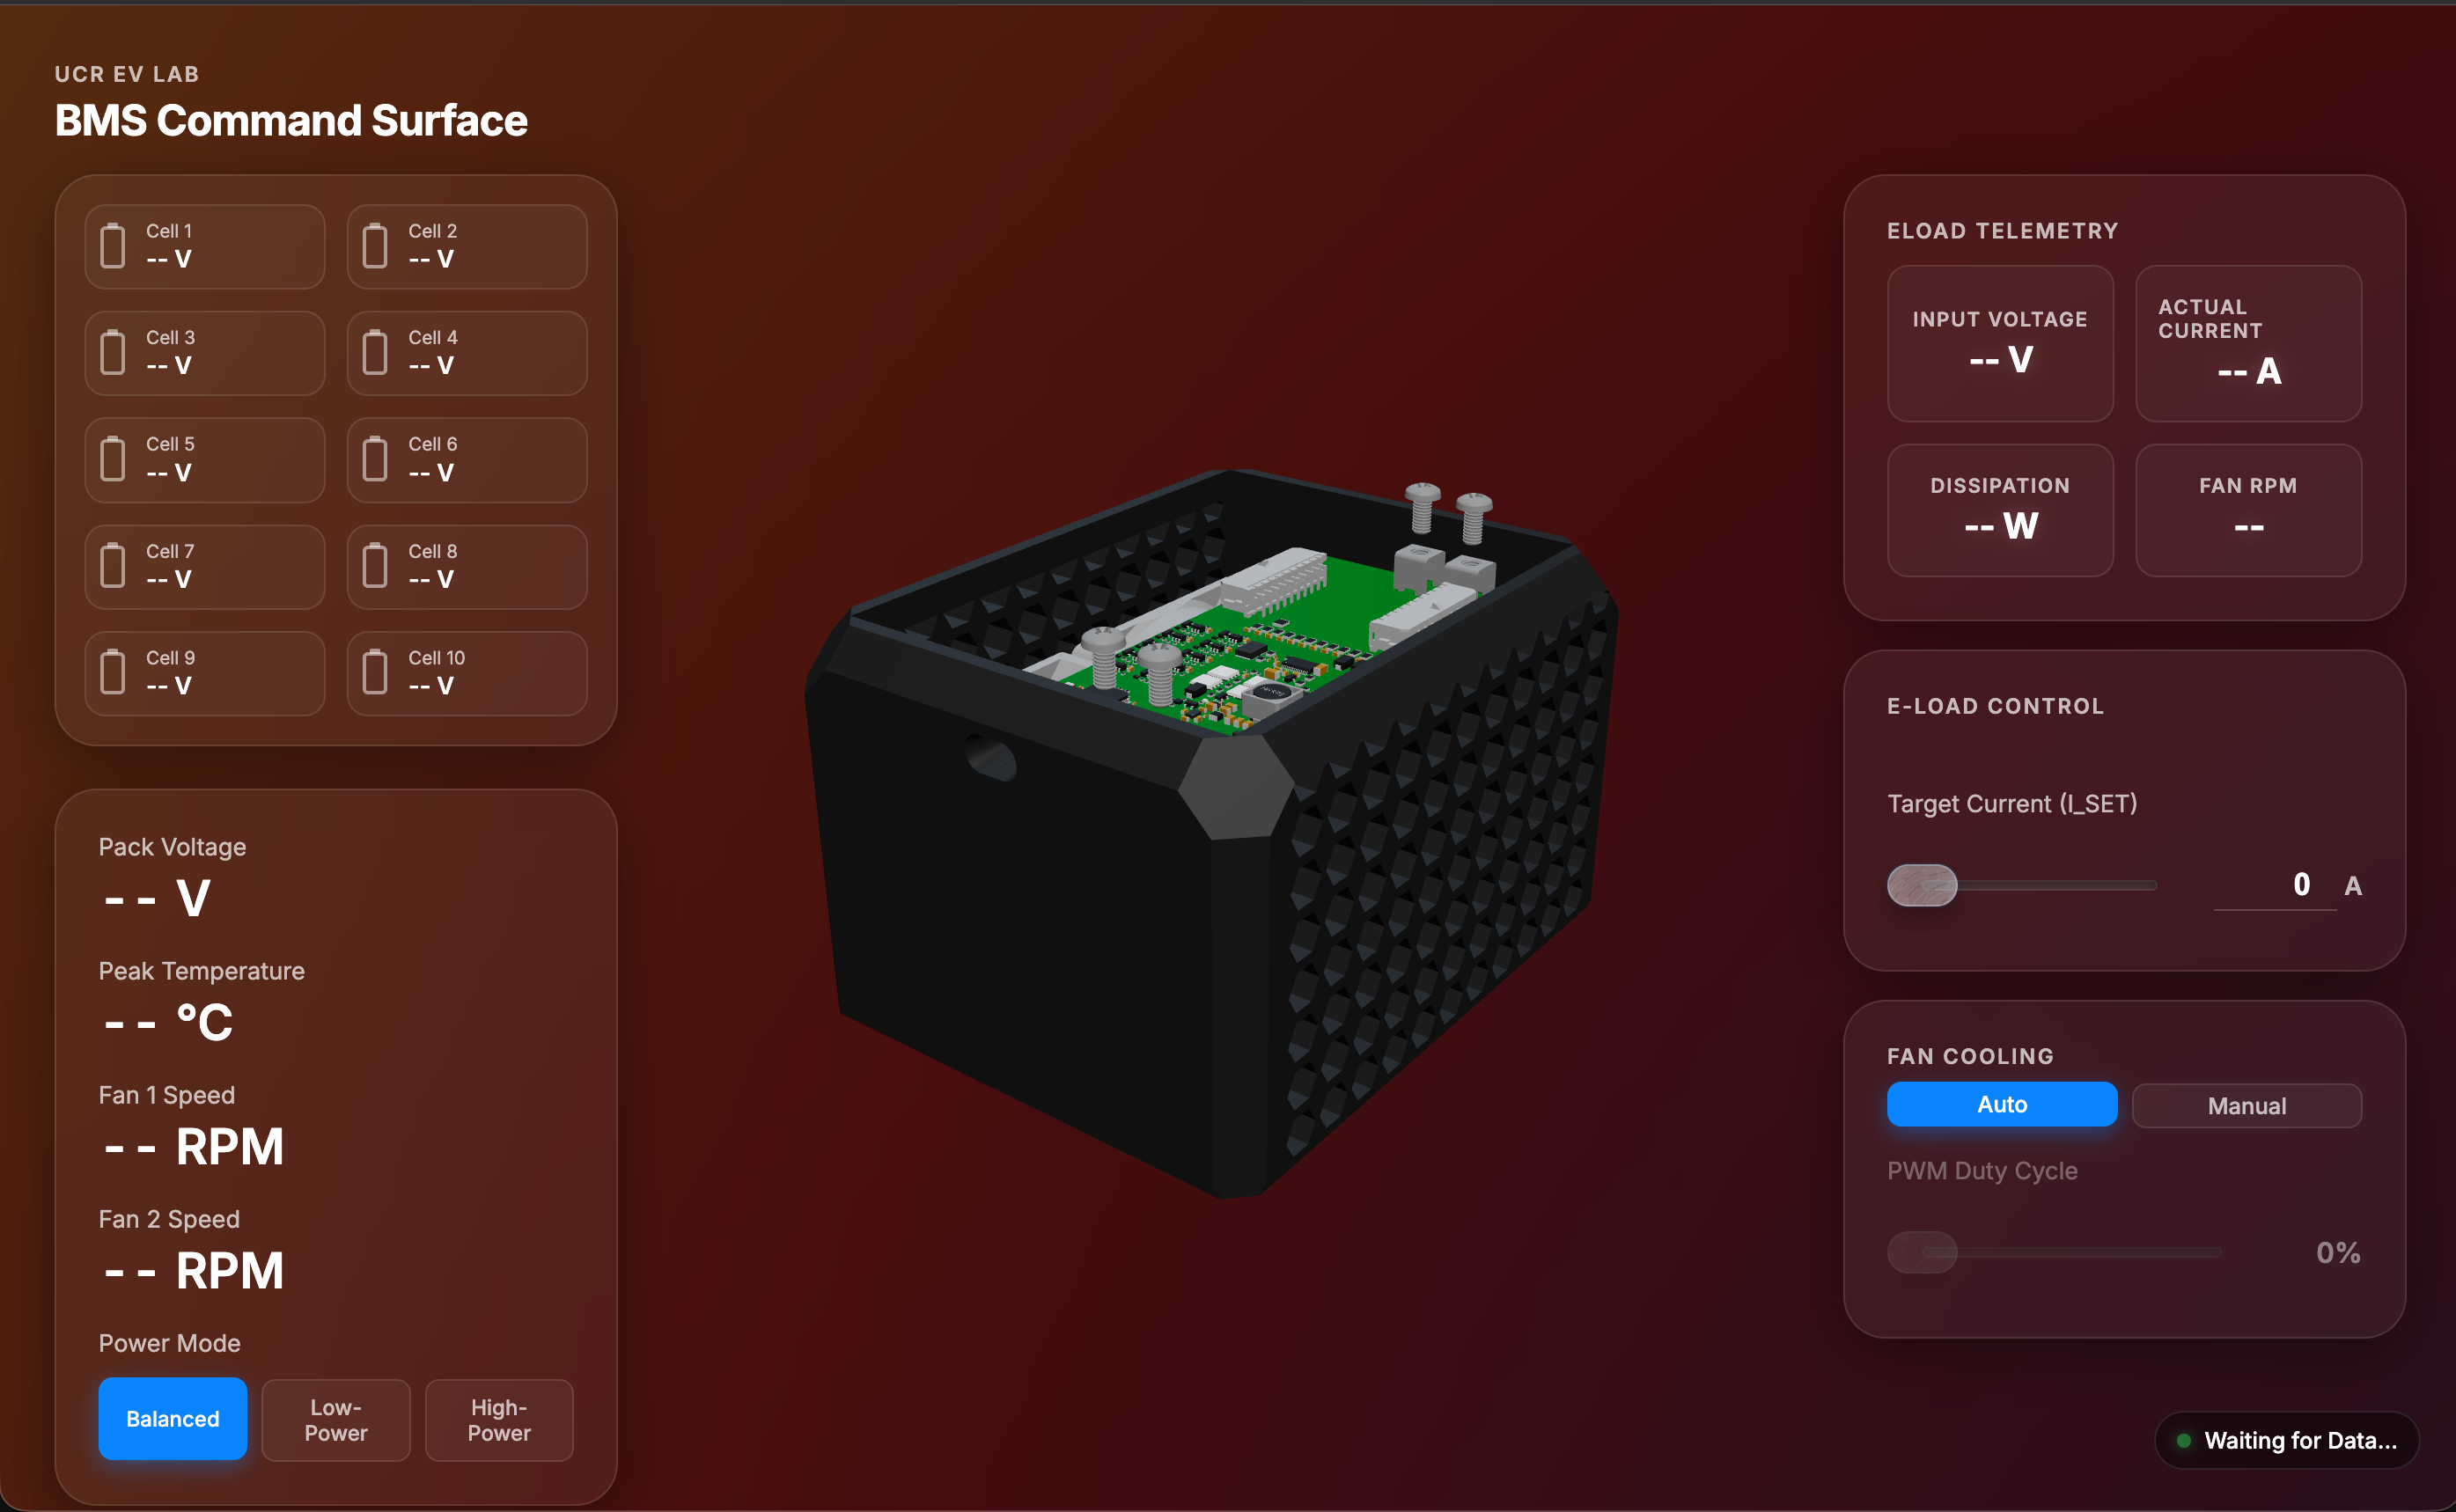
\includegraphics[width=0.95\textwidth]{BMS_GUI.png} [Figure 4]
\end{center}
\noindent
\textit{Figure D1:} Screenshot of the custom Python GUI displaying real-time BMS data, including individual cell voltages, pack voltage, current, and temperature readings.

\vspace{1em}

\section{Appendix E - Firmware Development}
\begin{center}
    
\includegraphics[width=0.95\textwidth]{firmware.png} [Figure 5]
\end{center}
\noindent
\textit{Figure E1:} USB-Connection-Firmware project in STM32CubeIDE showing HAL driver integration and peripheral initialization for the STM32F303RC microcontroller.

\vspace{1em}

\section{Appendix F - BMS Command Surface}
\begin{center}
    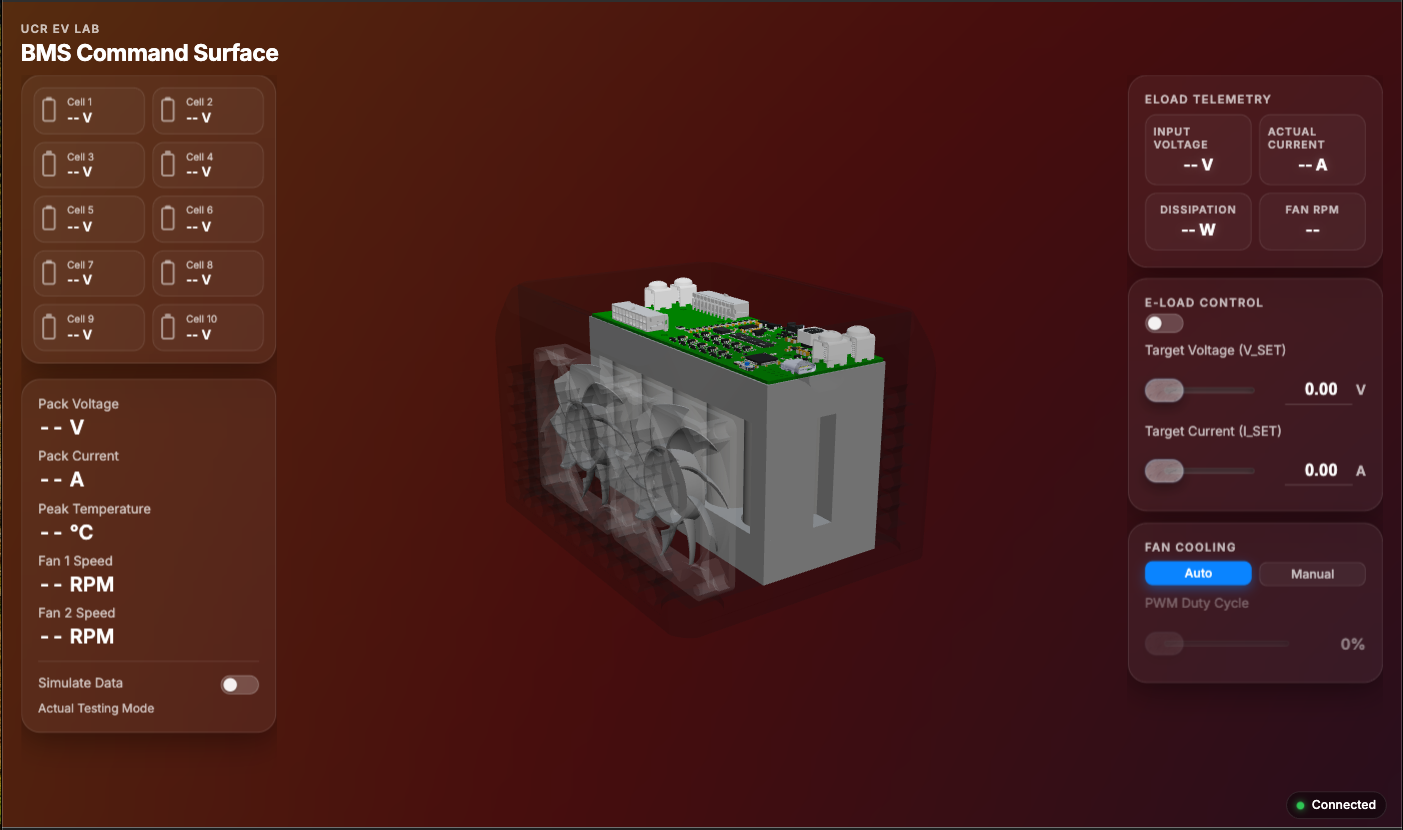
\includegraphics[width=0.95\textwidth]{2026-02-15_21-16-33.png} [Figure 6]
\end{center}
\noindent
\textit{Figure F1:} BMS Command Surface desktop application showing real-time cell voltage monitoring, pack telemetry, E-Load control interface, fan cooling management, and 3D enclosure visualization with simulation data toggle.

\end{document}
